\chapter{Sprint 2 : Modèles de classification des stades}
\label{chap:sprint2}

\sectionsansnum{Introduction}

Ce chapitre rend compte du deuxième sprint, consacré à l'entraînement des modèles de
classification. Le corpus produit au sprint précédent y est exploité pour entraîner
trois familles d'architectures sur quatre configurations, soit douze modèles au total.
Le sprint a été dominé par une contrainte matérielle qui a imposé un arbitrage explicite
sur la quantité de données exploitable, et dont la portée conditionne la lecture de tous
les résultats.

\section{Objectif du sprint}

L'objectif était de couvrir les \textbf{trois familles d'architectures} identifiées
comme complémentaires dans l'étude préalable, sur les \textbf{quatre configurations}
retenues : deux montages --- cinq dérivations pour le laboratoire, deux pour
l'ambulatoire --- et deux granularités de sortie --- trois stades pour la robustesse,
cinq pour la conformité au référentiel AASM.

Ce plan factoriel n'est pas gratuit. Il répond à une question que la littérature laisse
généralement ouverte : quelle est la part respective, dans la performance finale, de
l'architecture du modèle, du nombre de dérivations disponibles et de la granularité
demandée ? Entraîner les douze combinaisons permet d'y répondre par comparaison directe,
sur un protocole identique.

\section{Analyse du sprint 2}

\subsection{Sprint Backlog}

Le sprint a embarqué quatre récits pour 47 points de complexité
(tableau~\ref{tab:bl-s2}).

\begin{table}[H]
\centering\small
\renewcommand{\arraystretch}{1.15}
\begin{tabular}{@{}c|L{2.5cm}|L{4.6cm}|L{4.6cm}|c@{}}
\hline
\ligneentete \entete{ID} & \entete{Module} & \entete{R\'ecit utilisateur} & \entete{T\^aches} & \entete{Estim.} \\
\hline
\multirow{3}{*}{US-26} & \multirow{3}{=}{Corpus \`a l'\'echelle} & \multirow{3}{=}{En tant qu'ing\'enieur, je veux pr\'etraiter les 196 enregistrements de la cohorte clinique} & Rapatrier la cohorte apr\`es obtention de l'acc\`es & \multirow{3}{*}{8 pts} \\
 &  &  & Rejouer la cha\^ine de pr\'eparation \`a l'\'echelle &  \\
 &  &  & Contr\^oler la distribution des classes obtenue &  \\
\hline
\multirow{3}{*}{US-27} & \multirow{3}{=}{R\'eseau convolutif} & \multirow{3}{=}{En tant que syst\`eme, je veux classer chaque \'epoque avec un r\'eseau convolutif multi-\'echelle} & Concevoir les deux branches d'\'echelles distinctes & \multirow{3}{*}{13 pts} \\
 &  &  & Impl\'ementer la boucle d'entra\^inement &  \\
 &  &  & Entra\^iner les quatre variantes &  \\
\hline
\multirow{3}{*}{US-28} & \multirow{3}{=}{R\'eseau r\'ecurrent} & \multirow{3}{=}{En tant que syst\`eme, je veux classer chaque \'epoque avec un r\'eseau r\'ecurrent \`a pooling attentionnel} & Impl\'ementer le r\'eseau bidirectionnel \`a m\'emoire longue & \multirow{3}{*}{13 pts} \\
 &  &  & Ajouter le m\'ecanisme d'attention temporelle &  \\
 &  &  & Entra\^iner les quatre variantes &  \\
\hline
\multirow{3}{*}{US-29} & \multirow{3}{=}{R\'eseau attentionnel} & \multirow{3}{=}{En tant que syst\`eme, je veux classer chaque \'epoque avec un Transformer par patchs} & D\'ecouper l'\'epoque en fragments et les projeter & \multirow{3}{*}{13 pts} \\
 &  &  & Ajouter le jeton de synth\`ese et l'encodage positionnel &  \\
 &  &  & Entra\^iner les quatre variantes &  \\
\hline
\end{tabular}
\caption{Sprint Backlog --- Sprint 2}
\label{tab:bl-s2}
\end{table}

\subsection{Diagramme des cas d'utilisation}

Le cas d'utilisation de ce sprint reste porté par le moteur d'inférence
(figure~\ref{fig:uc-s2}). Le praticien n'y accède pas directement : il en bénéficiera au
sprint 4, lorsque le service d'inférence sera exposé.

\begin{figure}[H]
\centering
\begin{tikzpicture}[
    x=1cm,y=1cm,
    uc/.style     = {ellipse, draw=hypnoblue!60, fill=hypnolight,
                     align=center, font=\scriptsize, text width=2.7cm,
                     inner sep=1.5pt, minimum height=1.0cm},
    ucp/.style    = {ellipse, draw=hypnored!70, fill=hypnored!7,
                     align=center, font=\scriptsize\bfseries, text width=2.7cm,
                     inner sep=1.5pt, minimum height=1.0cm},
    lien/.style   = {hypnogray!75, line width=0.55pt},
    rel/.style    = {-{Latex[length=2mm]}, hypnoblue!70, line width=0.5pt, dashed},
    et/.style     = {font=\tiny\itshape, text=hypnoblue!85, fill=white, inner sep=1pt},
    nomact/.style = {font=\scriptsize\bfseries, align=center, text width=2.2cm},
  ]

  \tikzset{acteur/.pic={
      \draw[hypnoblue,line width=0.8pt] (0,0) circle (0.17);
      \draw[hypnoblue,line width=0.8pt] (0,-0.17) -- (0,-0.66);
      \draw[hypnoblue,line width=0.8pt] (-0.28,-0.34) -- (0.28,-0.34);
      \draw[hypnoblue,line width=0.8pt] (0,-0.66) -- (-0.24,-1.04);
      \draw[hypnoblue,line width=0.8pt] (0,-0.66) -- (0.24,-1.04);}}

  \draw[hypnoblue!55,line width=0.9pt,rounded corners=3pt]
       (3.1,-4.6) rectangle (12.5,2.4);
  \node[font=\small\bfseries,text=hypnoblue,anchor=north west] at (3.35,2.25)
       {Module de classification};

  \node[ucp] (cls) at (5.2, 0.9)  {Classer une\\époque};
  \node[uc]  (sel) at (5.2,-2.9)  {Choisir la\\configuration};

  \node[uc]  (cnn) at (10.1, 1.2) {Extraire les motifs\\multi-échelles};
  \node[uc]  (rec) at (10.1,-0.4) {Modéliser la\\dynamique temporelle};
  \node[uc]  (att) at (10.1,-2.0) {Pondérer les\\fragments par attention};
  \node[uc]  (pon) at (10.1,-3.6) {Pondérer les\\classes rares};

  \pic at (1.3,0.6) {acteur};
  \node[nomact,anchor=north] at (1.3,-0.05) {Moteur\\d'inférence};

  \draw[lien] (1.7,0.25) -- (cls.west);
  \draw[lien] (1.7,0.25) -- (sel.west);

  \draw[rel] (cls) -- node[et,pos=0.62] {$\ll$extend$\gg$} (cnn);
  \draw[rel] (cls) -- node[et,pos=0.62] {$\ll$extend$\gg$} (rec);
  \draw[rel] (cls) -- node[et,pos=0.64] {$\ll$extend$\gg$} (att);
  \draw[rel] (cls) -- node[et,pos=0.68] {$\ll$include$\gg$} (pon);

\end{tikzpicture}
\caption{Diagramme des cas d'utilisation du sprint 2 --- classification des stades}
\label{fig:uc-s2}
\end{figure}

\subsubsection{Description textuelle des cas d'utilisation}

\begin{casutilisation}{Description textuelle du cas « Classer une époque »}
Titre & Classer une époque \\ \hline
Acteur & Moteur d'inférence \\ \hline
Description & Attribuer à une fenêtre de 30 secondes le stade de vigilance qui la
caractérise, parmi trois ou cinq classes selon la configuration \\ \hline
Préconditions & Un tenseur d'époques normalisées est disponible ; le modèle
correspondant à la configuration demandée est chargé \\ \hline
Scénario de base &
\begin{minipage}[t]{\linewidth}
\begin{enumerate}[leftmargin=1.1em,itemsep=1pt,topsep=3pt]
  \item Le système sélectionne le modèle correspondant au montage et à la granularité.
  \item Il constitue des lots d'époques et les transfère au processeur graphique.
  \item Le modèle produit un vecteur de scores par époque.
  \item Le système retient la classe de score maximal.
  \item Il restitue la séquence de stades pour l'enregistrement complet.
\end{enumerate}
\end{minipage} \\ \hline
Scénario alternatif &
\begin{minipage}[t]{\linewidth}
\begin{itemize}[leftmargin=1.1em,itemsep=1pt,topsep=3pt]
  \item \textbf{1a} --- Le modèle demandé n'est pas disponible : l'opération est refusée
        avec un message explicite.
  \item \textbf{2a} --- La mémoire du processeur graphique est insuffisante : le
        traitement bascule sur le processeur central.
\end{itemize}
\end{minipage}
\end{casutilisation}

\subsection{Diagramme de séquence objet}

La figure~\ref{fig:seq-s2} décrit la boucle d'entraînement d'un modèle.

\begin{figure}[H]
\centering
\resizebox{0.96\textwidth}{!}{%
\begin{sequencediagram}
  \newthread[hypnolight]{e}{\scriptsize Boucle d'entraînement}
  \newinst[2.0]{c}{\scriptsize Corpus en mémoire}
  \newinst[2.0]{m}{\scriptsize Modèle}
  \newinst[2.0]{o}{\scriptsize Optimiseur}
  \newinst[2.2]{v}{\scriptsize Évaluateur}

  \begin{call}{e}{\scriptsize charger le corpus}{c}{\scriptsize tenseur complet}
  \end{call}
  \begin{sdblock}{\scriptsize loop}{\scriptsize 30 époques d'entraînement}
    \begin{sdblock}{\scriptsize loop}{\scriptsize sur chaque lot}
      \begin{call}{e}{\scriptsize transférer le lot}{c}{\scriptsize lot de 128}
      \end{call}
      \begin{call}{e}{\scriptsize propagation avant}{m}{\scriptsize scores}
      \end{call}
      \begin{call}{e}{\scriptsize perte pondérée}{o}{\scriptsize gradients}
      \end{call}
      \begin{call}{e}{\scriptsize écrêter et appliquer}{m}{}
      \end{call}
    \end{sdblock}
    \begin{call}{e}{\scriptsize évaluer sur validation}{v}{\scriptsize $\kappa$ de Cohen}
    \end{call}
    \begin{sdblock}{\scriptsize alt}{\scriptsize $\kappa$ amélioré}
      \begin{call}{e}{\scriptsize conserver le point de contrôle}{m}{}
      \end{call}
    \end{sdblock}
  \end{sdblock}
  \begin{call}{e}{\scriptsize évaluer sur test}{v}{\scriptsize métriques finales}
  \end{call}
\end{sequencediagram}}
\caption{Diagramme de séquence objet du sprint 2 --- entraînement d'un modèle}
\label{fig:seq-s2}
\end{figure}

\section{Réalisation}

\subsection{Les trois architectures}

\subsubsection{Réseau convolutif multi-échelle}

Le premier modèle exploite une observation issue de l'étude préalable : les éléments
graphiques du référentiel AASM vivent à des échelles temporelles différentes. Un fuseau
du sommeil dure environ une demi-seconde et oscille autour de 12 à 14 hertz ; une onde
lente s'étale sur plus d'une seconde. Un noyau de convolution unique ne peut capter les
deux.

L'architecture retenue comporte donc deux branches parallèles appliquées au même signal
(figure~\ref{fig:cnn}). La branche fine emploie un noyau de 50 échantillons --- une
demi-seconde --- et la branche grossière un noyau de 200 échantillons, soit deux
secondes. Leurs représentations sont concaténées avant classification.

\begin{figure}[H]
\centering
\begin{tikzpicture}[
    x=1cm,y=1cm,
    bl/.style   = {rectangle,rounded corners=2pt,draw=hypnoblue!60,fill=hypnolight,
                   align=center,font=\tiny,minimum height=0.95cm,text width=2.0cm},
    blf/.style  = {rectangle,rounded corners=2pt,draw=hypnored!65,fill=hypnored!7,
                   align=center,font=\tiny,minimum height=0.95cm,text width=2.0cm},
    io/.style   = {rectangle,rounded corners=2pt,draw=hypnogray!60,fill=white,
                   align=center,font=\tiny,minimum height=0.95cm,text width=1.9cm},
    fl/.style   = {-{Latex[length=1.8mm]},hypnoblue!75,line width=0.7pt},
    tag/.style  = {font=\tiny\itshape,text=hypnogray},
  ]

  \node[io] (in) at (0,0) {Entrée\\$(C, 3000)$};

  \node[bl] (f1) at (3.0, 1.35) {Conv 1D\\noyau 50, pas 6};
  \node[bl] (f2) at (5.6, 1.35) {Sous-échant.\\$\times 4$};
  \node[bl] (f3) at (8.2, 1.35) {Conv 1D\\noyau 8};
  \node[bl] (f4) at (10.8,1.35) {Moyennage\\adaptatif $\to 16$};

  \node[bl] (g1) at (3.0,-1.35) {Conv 1D\\noyau 200, pas 25};
  \node[bl] (g2) at (5.6,-1.35) {Sous-échant.\\$\times 4$};
  \node[bl] (g3) at (8.2,-1.35) {Conv 1D\\noyau 8};
  \node[bl] (g4) at (10.8,-1.35) {Moyennage\\adaptatif $\to 16$};

  \node[blf] (cat) at (13.3,0) {Concaténation\\$4096$};
  \node[io]  (out) at (13.3,-2.1) {Logits\\$(K)$};

  \foreach \a/\b in {f1/f2,f2/f3,f3/f4,g1/g2,g2/g3,g3/g4} \draw[fl] (\a) -- (\b);
  \draw[fl] (in) |- (f1);
  \draw[fl] (in) |- (g1);
  \draw[fl] (f4) -| (cat);
  \draw[fl] (g4) -| (cat);
  \draw[fl] (cat) -- node[tag,right,pos=0.5] {\ 3 couches denses} (out);

  \node[tag,anchor=west] at (1.35, 1.95) {branche fine --- 0,5\,s};
  \node[tag,anchor=west] at (1.35,-1.95) {branche grossière --- 2\,s};

\end{tikzpicture}
\vspace{0.3cm}
\caption[Architecture du réseau convolutif]%
        {Réseau convolutif à deux branches d'échelles temporelles distinctes.}
\label{fig:cnn}
\end{figure}

\subsubsection{Réseau récurrent à pooling attentionnel}

Le deuxième modèle traite l'époque comme une séquence de \num{3000} pas, chacun décrit
par les dérivations disponibles. Un réseau récurrent bidirectionnel à mémoire
longue~\cite{hochreiter1997}, de deux couches de 128 unités, en produit une
représentation contextualisée dans les deux sens du temps.

Se pose alors la question de la réduction : comment condenser \num{3000} états en un
vecteur unique ? Prendre le dernier état privilégierait la fin de la fenêtre ; en faire
la moyenne diluerait un événement bref dans le reste. Nous employons un \textbf{pooling
attentionnel}~\cite{bahdanau2015} : un petit réseau apprend à attribuer à chaque pas un
poids, dont la somme vaut un, et la représentation finale est la moyenne pondérée des
états (figure~\ref{fig:lstm}).

\begin{figure}[H]
\centering
\begin{tikzpicture}[
    x=1cm,y=1cm,
    bl/.style   = {rectangle,rounded corners=2pt,draw=hypnoblue!60,fill=hypnolight,
                   align=center,font=\tiny,minimum height=1.0cm,text width=2.3cm},
    blf/.style  = {rectangle,rounded corners=2pt,draw=hypnored!65,fill=hypnored!7,
                   align=center,font=\tiny,minimum height=1.0cm,text width=2.3cm},
    io/.style   = {rectangle,rounded corners=2pt,draw=hypnogray!60,fill=white,
                   align=center,font=\tiny,minimum height=1.0cm,text width=2.0cm},
    fl/.style   = {-{Latex[length=1.8mm]},hypnoblue!75,line width=0.7pt},
    tag/.style  = {font=\tiny\itshape,text=hypnogray,align=center},
  ]

  \node[io] (in)  at (0,0)    {Séquence\\$(3000, C)$};
  \node[bl] (l1)  at (3.1,0)  {LSTM bidirectionnel\\2 couches $\times$ 128};
  \node[bl] (st)  at (6.4,0)  {États contextualisés\\$(3000, 256)$};
  \node[blf](at)  at (9.7,0)  {Pooling attentionnel\\$\sum_t \alpha_t h_t$};
  \node[bl] (fc)  at (12.9,0) {Couches denses\\$256 \to 64 \to K$};

  \foreach \a/\b in {in/l1,l1/st,st/at,at/fc} \draw[fl] (\a) -- (\b);

  \node[bl,minimum height=0.75cm,text width=2.3cm] (sc) at (9.7,-1.9)
       {Scores $\alpha_t$\\\tiny normalisés, de somme 1};
  \draw[fl] (st) |- (sc);
  \draw[fl] (sc) -- (at);

  \node[tag,anchor=north,text width=6.5cm] at (6.4,-2.35)
       {les poids d'attention indiquent les instants retenus};

\end{tikzpicture}
\vspace{0.3cm}
\caption[Architecture du réseau récurrent]%
        {Réseau récurrent bidirectionnel à pooling attentionnel.}
\label{fig:lstm}
\end{figure}

\subsubsection{Réseau attentionnel par patchs}

Le troisième modèle abandonne la récurrence au profit de l'auto-attention~\cite{vaswani2017}.
L'époque est découpée en 60 fragments consécutifs de 50 échantillons, chacun projeté
linéairement dans un espace de dimension 128. Un jeton de synthèse est ajouté en tête de
séquence, et un encodage positionnel sinusoïdal réinjecte l'ordre temporel que
l'auto-attention, par construction, ignore (figure~\ref{fig:transformer}).

Le découpage en fragments est ce qui rend l'approche viable. L'auto-attention a un coût
quadratique en la longueur de séquence : l'appliquer aux \num{3000} échantillons bruts
demanderait neuf millions de coefficients par tête et par époque. Ramenée à 61 jetons,
la même opération en demande moins de quatre mille.

\begin{figure}[H]
\centering
\begin{tikzpicture}[
    x=1cm,y=1cm,
    bl/.style   = {rectangle,rounded corners=2pt,draw=hypnoblue!60,fill=hypnolight,
                   align=center,font=\tiny,minimum height=1.0cm,text width=2.25cm},
    blf/.style  = {rectangle,rounded corners=2pt,draw=hypnored!65,fill=hypnored!7,
                   align=center,font=\tiny,minimum height=1.0cm,text width=2.25cm},
    io/.style   = {rectangle,rounded corners=2pt,draw=hypnogray!60,fill=white,
                   align=center,font=\tiny,minimum height=1.0cm,text width=1.95cm},
    fl/.style   = {-{Latex[length=1.8mm]},hypnoblue!75,line width=0.7pt},
    tag/.style  = {font=\tiny\itshape,text=hypnogray,align=center},
  ]

  \node[io]  (in)  at (0,0)    {Entrée\\$(C, 3000)$};
  \node[bl]  (pa)  at (2.9,0)  {Découpage\\60 fragments de 50};
  \node[bl]  (pe)  at (5.9,0)  {Projection linéaire\\$\to 128$};
  \node[blf] (cls) at (8.9,0)  {Jeton de synthèse\\et encodage positionnel};
  \node[bl]  (tr)  at (11.9,0) {Encodeur\\4 couches, 8 têtes};
  \node[io]  (out) at (11.9,-2.0) {Logits\\$(K)$};

  \foreach \a/\b in {in/pa,pa/pe,pe/cls,cls/tr} \draw[fl] (\a) -- (\b);
  \draw[fl] (tr) -- node[tag,right,pos=0.5,text width=2.4cm]
                    {\ classification sur le jeton de synthèse} (out);

  \node[tag,anchor=north,text width=5.0cm] at (4.4,-1.05)
       {coût quadratique ramené de $3000^2$ à $61^2$};

\end{tikzpicture}
\vspace{0.3cm}
\caption[Architecture du modèle attentionnel]%
        {Modèle attentionnel : l'époque est traitée comme une suite de fragments.}
\label{fig:transformer}
\end{figure}

\subsection{Stratégie d'entraînement sous contrainte matérielle}

\subsubsection{Dimensionnement du problème}

Une époque de 30 secondes échantillonnée à \SI{100}{\hertz} sur cinq dérivations occupe
\SI{60}{\kilo\octet} en simple précision. Rapporté à une cohorte entière, le corpus
dépasse de plusieurs ordres de grandeur ce qu'une station de développement peut contenir
(tableau~\ref{tab:empreinte}).

\begin{table}[H]
\centering

\small
\begin{tabular}{@{}L{5.0cm}rrrl@{}}
\toprule
\textbf{Configuration} & \textbf{Sujets} & \textbf{Époques} & \textbf{Empreinte} &
\textbf{Tient dans} \\
\midrule
2 dérivations & 196 & \num{195130} & \SI{4,7}{\giga\octet} & mémoire vidéo et vive \\
5 dérivations & 196 & \num{195130} & \SI{11,7}{\giga\octet} & mémoire vive seulement \\
5 dérivations, variante attentionnelle & 150 & \num{148958} & \SI{8,9}{\giga\octet} &
mémoire vive seulement \\
\textbf{cohorte SHHS1 complète} & \num{5793} & $\approx$ \num{5800000} &
$\approx$ \SI{346}{\giga\octet} & ni l'une ni l'autre \\
\bottomrule
\end{tabular}
\caption{Empreinte du corpus d'entraînement en simple précision}
\label{tab:empreinte}
\end{table}

La cohorte complète représenterait environ \SI{346}{\giga\octet}. Comme les fichiers
préparés sont stockés exactement tels qu'ils seront chargés, ce chiffre vaut aussi bien
pour le disque que pour la mémoire : la contrainte se manifeste deux fois, dès la
préparation. La question n'est donc pas « toutes les données ou pas », mais \emph{quelle
fraction} convertir et \emph{comment} la faire circuler jusqu'au processeur graphique.

\subsubsection{Trois stratégies de résidence des données}

\begin{table}[H]
\centering

\small
\begin{tabular}{@{}L{2.9cm}L{4.5cm}L{4.3cm}c@{}}
\toprule
\textbf{Stratégie} & \textbf{Principe} & \textbf{Limite} & \textbf{Décision} \\
\midrule
Tout en mémoire vidéo &
Le corpus est transféré une fois sur le processeur graphique ; plus aucune copie
pendant l'entraînement &
Ne laisse pas de marge pour les activations et exclut d'emblée le protocole à cinq
dérivations & écartée \\
\addlinespace[3pt]
\textbf{Tout en mémoire vive} &
Le corpus réside dans la mémoire de l'hôte ; chaque lot est copié vers le processeur
graphique en accès direct depuis une zone page-verrouillée &
Plafonne le nombre de sujets ; empreinte doublée au moment du découpage &
\textbf{retenue} \\
\addlinespace[3pt]
Lecture paresseuse &
Chaque lot est relu sur disque à la volée ; l'empreinte mémoire devient négligeable &
Le processeur graphique attend le disque à chaque itération &
écartée \\
\bottomrule
\end{tabular}
\caption{Stratégies de résidence des données pendant l'entraînement}
\label{tab:residence}
\end{table}

La lecture paresseuse aurait permis d'exploiter les \num{5793} enregistrements, mais en
affamant le processeur graphique : le temps par époque devient dominé par les
entrées-sorties. Dans les quatre semaines du sprint, il aurait fallu descendre bien en
dessous des trente époques d'entraînement nécessaires à la convergence, et cela pour
douze variantes. Le modèle aurait vu davantage de patients, mais chacun beaucoup moins
souvent, et aurait sous-appris.

Le choix inverse a été fait : \textbf{restreindre la cohorte à 196 sujets pour que le
corpus tienne intégralement en mémoire vive}, et consacrer la totalité du budget de
calcul à l'apprentissage plutôt qu'au transfert. Les \num{195130} exemples étiquetés
restent largement suffisants pour des architectures de quelques millions de paramètres,
et les trente époques complètes ont pu être menées sur les douze variantes.

\subsubsection{La contrainte était réelle}

Onze carnets sur douze fixent la limite à 196 sujets. Le douzième --- le modèle
attentionnel à cinq dérivations et trois classes --- descend à \textbf{150}, soit
\num{148958} époques et \SI{8,9}{\giga\octet}. Ce modèle matérialise soixante jetons de
dimension 128 par époque, ainsi qu'une matrice d'attention par tête : ses activations
débordaient là où les deux autres architectures passaient encore.

Cette réduction explique un écart qu'il faut signaler pour qu'il ne passe pas pour une
erreur : le jeu de test de cette seule variante compte \num{14896} époques au lieu de
\num{19513}.

\subsubsection{Réglages d'entraînement}

\begin{table}[H]
\centering

\small
\begin{tabular}{@{}L{4.0cm}L{10.0cm}@{}}
\toprule
\textbf{Réglage} & \textbf{Effet recherché} \\
\midrule
Précision mixte & Activations en demi-précision, accumulations en simple précision,
avec mise à l'échelle des gradients : environ deux fois moins de mémoire
d'activations et un gain de débit sur les unités tensorielles \\
\addlinespace[2pt]
Mémoire page-verrouillée & Copie en accès direct vers le processeur graphique,
recouvrant le calcul du lot précédent \\
\addlinespace[2pt]
Aucun processus de chargement parallèle & Choix contre-intuitif mais adapté : les
données étant déjà en mémoire, un processus supplémentaire dupliquerait le tenseur de
\SI{11,7}{\giga\octet} sans rien précharger \\
\addlinespace[2pt]
Segments extensibles & Limite la fragmentation de l'allocateur, source d'échecs
d'allocation en fin d'entraînement \\
\addlinespace[2pt]
Optimiseur AdamW, pas initial \num{5e-4} & Découplage de la régularisation et de
l'adaptation du pas \\
\addlinespace[2pt]
Recuit cosinus sur 30 époques & Décroissance progressive du pas jusqu'à \num{1e-6} \\
\addlinespace[2pt]
Écrêtage du gradient à \num{1,0} & Indispensable au modèle récurrent, où les gradients
explosent sur des séquences de \num{3000} pas \\
\addlinespace[2pt]
Sélection sur le $\kappa$ de validation & Sur des classes déséquilibrées, la perte peut
s'améliorer pendant que la classe minoritaire se dégrade ; le $\kappa$ de
Cohen~\cite{cohen1960} ne le permet pas \\
\bottomrule
\end{tabular}
\caption{Réglages d'entraînement}
\label{tab:optim}
\end{table}

La figure~\ref{fig:courbes} illustre le déroulement d'un entraînement. L'écart croissant
entre les courbes d'entraînement et de validation traduit un surapprentissage progressif,
que la sélection du meilleur point de contrôle sur le $\kappa$ de validation neutralise
en pratique.

\begin{figure}[H]
\centering
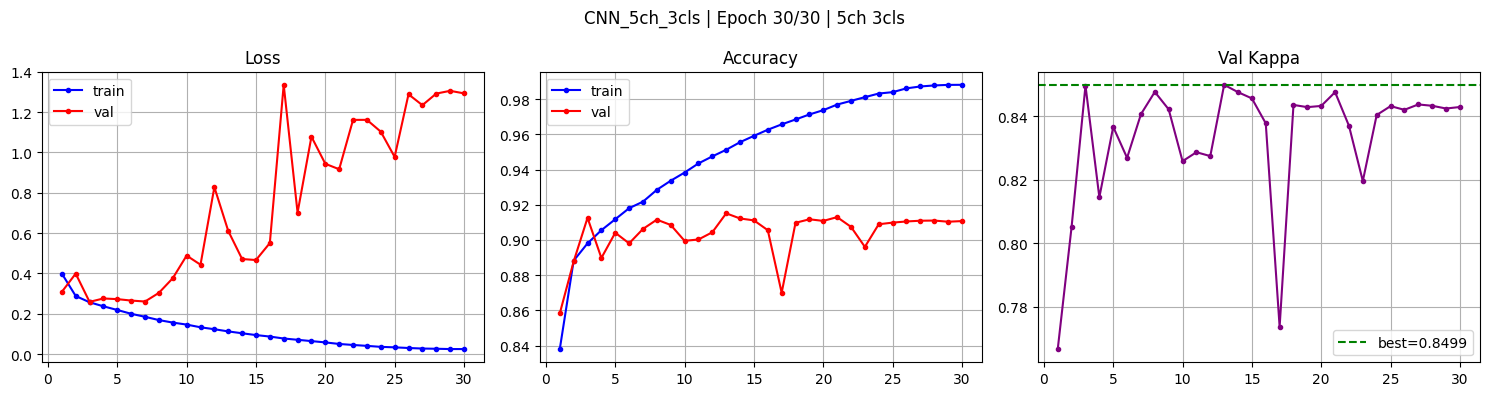
\includegraphics[width=\textwidth]{images/resultats/curves_CNN_5ch_3cls.png}
\caption[Courbes d'apprentissage du modèle convolutif]%
        {Évolution de la perte, de l'exactitude et du $\kappa$ de validation au cours
         des trente époques d'entraînement du modèle convolutif à cinq dérivations et
         trois classes.}
\label{fig:courbes}
\end{figure}

\subsection{Résultats}

\subsubsection{Les douze modèles}

\begin{table}[H]
\centering

\small
\begin{tabular}{@{}llcccc@{}}
\toprule
\textbf{Configuration} & \textbf{Architecture} & \textbf{Exactitude} &
\textbf{$\kappa$} & \textbf{F1 macro} & \textbf{F1 pondéré} \\
\midrule
\multirow{3}{*}{5 dérivations, 3 classes}
 & Convolutif   & \textbf{\SI{91,66}{\percent}} & \textbf{0,853} & 0,89 & 0,92 \\
 & Récurrent    & \SI{90,86}{\percent} & 0,843 & 0,89 & 0,91 \\
 & Attentionnel & \SI{90,14}{\percent} & 0,826 & 0,87 & 0,90 \\
\midrule
\multirow{3}{*}{2 dérivations, 3 classes}
 & Convolutif   & \SI{89,10}{\percent} & 0,810 & 0,86 & 0,89 \\
 & Récurrent    & \SI{87,58}{\percent} & 0,790 & 0,84 & 0,88 \\
 & Attentionnel & \SI{86,92}{\percent} & 0,771 & 0,83 & 0,87 \\
\midrule
\multirow{3}{*}{5 dérivations, 5 classes}
 & Convolutif   & \SI{82,78}{\percent} & 0,761 & 0,72 & 0,83 \\
 & Récurrent    & \SI{78,60}{\percent} & 0,713 & 0,71 & 0,80 \\
 & Attentionnel & \SI{81,55}{\percent} & 0,742 & 0,70 & 0,81 \\
\midrule
\multirow{3}{*}{2 dérivations, 5 classes}
 & Convolutif   & \SI{79,90}{\percent} & 0,723 & 0,69 & 0,80 \\
 & Récurrent    & \SI{76,01}{\percent} & 0,679 & 0,68 & 0,78 \\
 & Attentionnel & \SI{77,15}{\percent} & 0,686 & 0,66 & 0,77 \\
\bottomrule
\end{tabular}
\caption{Performances des douze modèles de base sur le jeu de test}
\label{tab:12modeles}
\end{table}

Trois enseignements se dégagent.

\paragraph{L'apport des dérivations oculaires et musculaires est net.} À granularité
constante, le passage de deux à cinq dérivations gagne entre \num{2,6} et \num{3,9}
points d'exactitude. Ce résultat était attendu : l'électro-oculogramme et
l'électromyogramme portent précisément l'information qui distingue le sommeil paradoxal.

\paragraph{Le passage à cinq stades coûte cher.} La même architecture perd entre
\num{8,6} et \num{12,3} points en passant de trois à cinq classes.

\paragraph{Le convolutif domine, mais de peu.} Il arrive en tête sur les quatre
configurations. L'écart avec les deux autres architectures reste toutefois inférieur à
quatre points, ce qui confirme qu'aucune famille ne domine franchement, et surtout que
leurs erreurs ne sont pas identiques.

La figure~\ref{fig:cm-3archi} rend cette dernière affirmation visible : les trois
matrices portent sur le même jeu de test, mais leurs erreurs ne se situent pas aux mêmes
endroits. C'est cette complémentarité que l'empilement, au sprint suivant, exploitera.

\begin{figure}[H]
\centering
\begin{subfigure}[t]{0.325\textwidth}
  \centering
  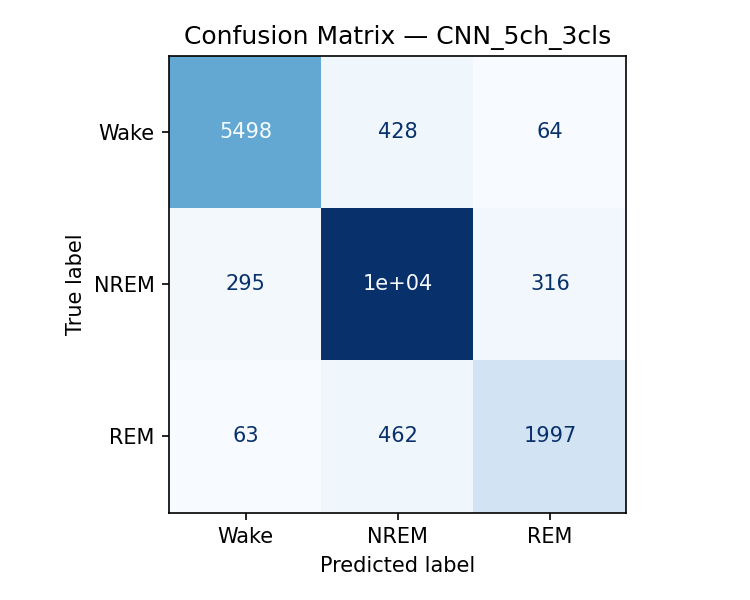
\includegraphics[width=\linewidth]{images/resultats/cm_CNN_5ch_3cls.png}
  \caption{Convolutif}
\end{subfigure}
\hfill
\begin{subfigure}[t]{0.325\textwidth}
  \centering
  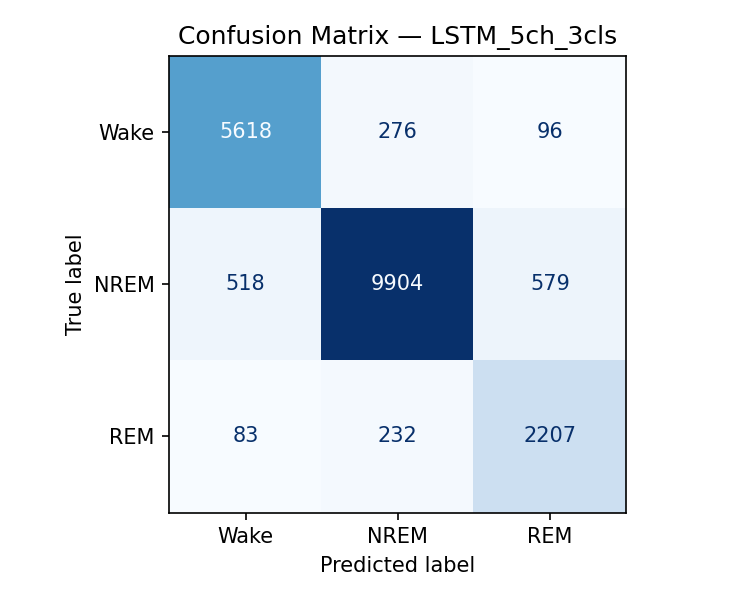
\includegraphics[width=\linewidth]{images/resultats/cm_LSTM_5ch_3cls.png}
  \caption{Récurrent}
\end{subfigure}
\hfill
\begin{subfigure}[t]{0.325\textwidth}
  \centering
  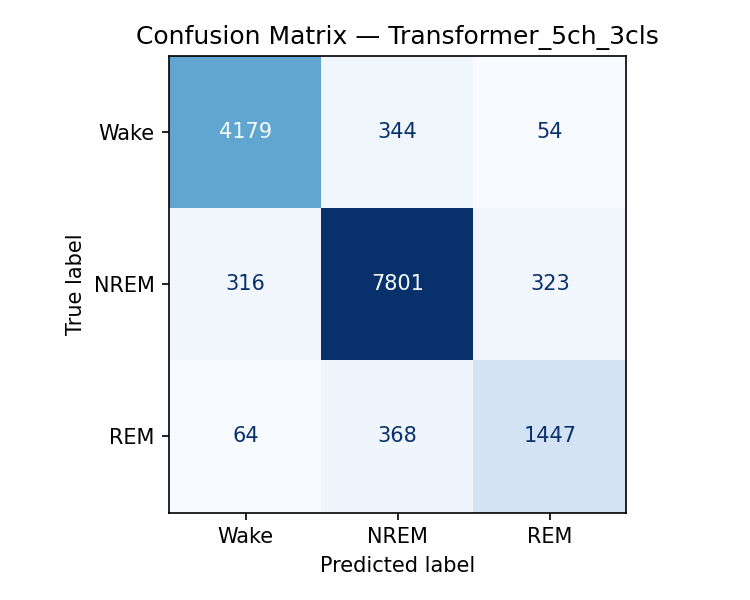
\includegraphics[width=\linewidth]{images/resultats/cm_Transformer_5ch_3cls.png}
  \caption{Attentionnel}
\end{subfigure}
\caption[Matrices de confusion des trois architectures]%
        {Matrices de confusion des trois architectures, configuration à cinq
         dérivations et trois classes. Effectifs bruts.}
\label{fig:cm-3archi}
\end{figure}

\subsubsection{Le problème du stade N1}

\begin{table}[H]
\centering

\small
\begin{tabular}{@{}llcccc@{}}
\toprule
& \textbf{Classe} & \textbf{Précision} & \textbf{Rappel} & \textbf{F1} &
\textbf{Effectif} \\
\midrule
\multirow{3}{*}{\rotatebox{90}{\scriptsize 3 classes}}
 & Éveil & 0,94 & 0,92 & 0,93 & \num{5990} \\
 & NREM  & 0,92 & 0,94 & 0,93 & \num{11001} \\
 & REM   & 0,84 & 0,79 & 0,82 & \num{2522} \\
\midrule
\multirow{5}{*}{\rotatebox{90}{\scriptsize 5 classes}}
 & Éveil & 0,92 & 0,92 & 0,92 & \num{5990} \\
 & N1    & \textcolor{hypnored}{\textbf{0,29}} &
           \textcolor{hypnored}{\textbf{0,24}} &
           \textcolor{hypnored}{\textbf{0,26}} & \num{638} \\
 & N2    & 0,86 & 0,78 & 0,82 & \num{7832} \\
 & N3    & 0,70 & 0,88 & 0,78 & \num{2531} \\
 & REM   & 0,80 & 0,84 & 0,82 & \num{2522} \\
\bottomrule
\end{tabular}
\caption{Performances par classe --- configuration à cinq dérivations}
\label{tab:parclasse}
\end{table}

Le constat est sans appel : \textbf{le stade N1 est la seule classe véritablement
échouée}, avec un F1 de \num{0,26} pour le modèle convolutif. Les autres architectures ne
font pas mieux --- le récurrent atteint \num{0,30} et l'attentionnel \num{0,21} --- mais
elles échouent différemment. Le récurrent affiche un rappel de \num{0,59} pour une
précision de \num{0,20} : il sur-prédit massivement le N1. Le convolutif fait l'inverse,
avec un rappel de \num{0,24} pour une précision de \num{0,29}.

La figure~\ref{fig:cm-5cls} montre où partent les époques de N1 mal classées.

\begin{figure}[H]
\centering
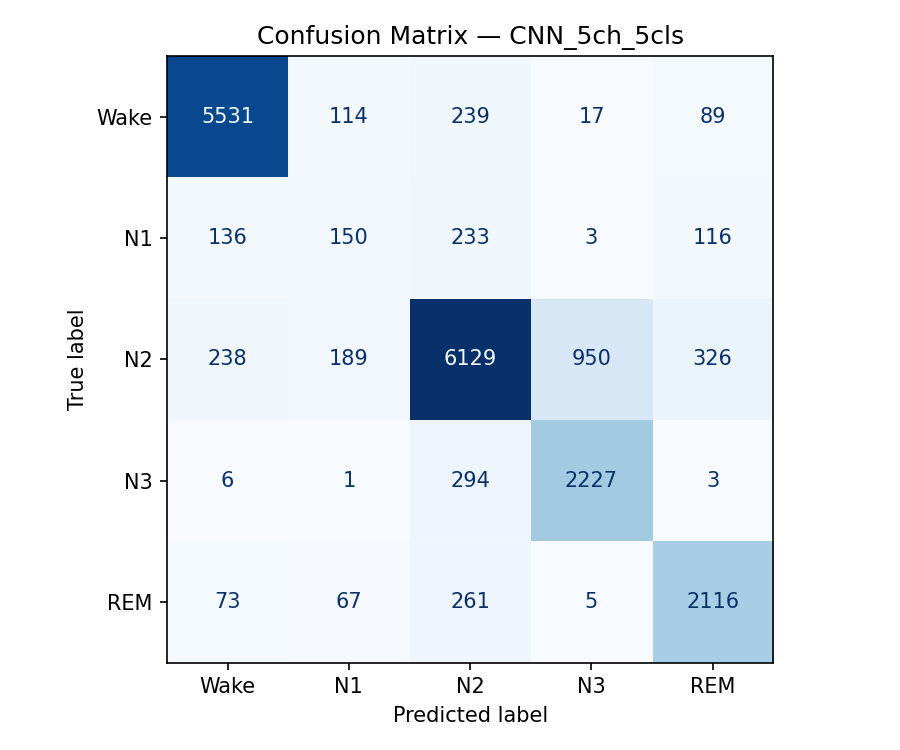
\includegraphics[width=0.72\textwidth]{images/resultats/cm_CNN_5ch_5cls.png}
\caption[Matrice de confusion à cinq classes]%
        {Matrice de confusion du modèle convolutif à cinq dérivations et cinq
         classes. Effectifs bruts sur les \num{19513} époques de test.}
\label{fig:cm-5cls}
\end{figure}

Sur les \num{638} époques réellement en N1, \num{150} seulement sont reconnues. Les
autres se dispersent : \num{233} sont versées en N2, \num{136} en éveil et \num{116} en
sommeil paradoxal. Cette dispersion n'est pas un défaut d'apprentissage mais le reflet de
la définition même du stade --- un état de transition sans marqueur graphique propre. Le
modèle le classe dans les états qui l'encadrent, ce que fait aussi un scoreur humain
hésitant.

On observe par ailleurs une seconde confusion, de nature différente : \num{950} époques
de N2 sont classées en N3. Celle-ci relève d'un seuil et non d'une ambiguïté --- le
référentiel AASM fixe le passage en N3 à \SI{20}{\percent} d'ondes lentes dans la
fenêtre, et une époque à \SI{19}{\percent} est presque indiscernable d'une époque à
\SI{21}{\percent}.

\sectionsansnum{Conclusion}

Ce sprint a produit douze modèles de classification couvrant trois architectures, deux
montages et deux granularités. La meilleure variante --- le réseau convolutif à cinq
dérivations et trois classes --- atteint \SI{91,66}{\percent} d'exactitude pour un
$\kappa$ de \num{0,853}, au voisinage de l'accord inter-expert rapporté dans la
littérature.

Le sprint a surtout imposé un arbitrage explicite : restreindre la cohorte pour maintenir
le corpus en mémoire vive, et préserver ainsi la qualité de convergence plutôt que le
volume de données. Cet arbitrage sera rediscuté dans la synthèse méthodologique du sprint
suivant.

Enfin, l'analyse par classe a révélé que les trois architectures échouent différemment sur
le stade N1. C'est précisément la condition d'efficacité de la combinaison de modèles, que
le sprint 3 met en œuvre.
